\begin{appendices}

\chapter{}

\enlargethispage{\baselineskip}
%\enlargethispage{\baselineskip}
\section{Extensión de la Herramienta IDA}

La herramienta Identifier Analyzer (IDA) posee una característica adicional. Dicha característica permite recibir como parámetro un archivo XML
%\footnote[1]{La ruta del archivo en un sistema de archivos de un sistema operativo determinado.} 
(Extensible Markup Language). Este archivo debe contener información asociada a identificadores (ids), literales y comentarios (propia de una aplicación JAVA).
%; esta información es similar a la que es capturada por el Analizador Sintáctico que IDA posee (Módulo de Extracción de Datos - Ver Capítulo 4).
La herramienta IDA lee la información provista por el archivo xml y ejecuta directamente los algoritmos de análisis de ids que tiene implementados. Por último, los resultados de la ejecución se almacenan en otro archivo XML que será creado en la misma ruta que el archivo leído como entrada \mbox{(Ver Figura \ref{arq1}).}

IDA soporta integración por medio de archivos XML. Esta característica es una ventaja que posibilita, compartir información con otras aplicaciones (herramientas) sin tener problemas de compatibilidad, dado que los archivos XML permiten un intercambio de datos estándar entre aplicaciones. De esta forma, IDA puede formar parte de un proceso de análisis más extenso que involucre otras herramientas asociadas a la comprensión de sistemas.

\vspace{-0.5em}

\begin{figure}[h!] %[h] para here [b] para bottom [t] para top
\centerline{%queda centrada mejor la imagen
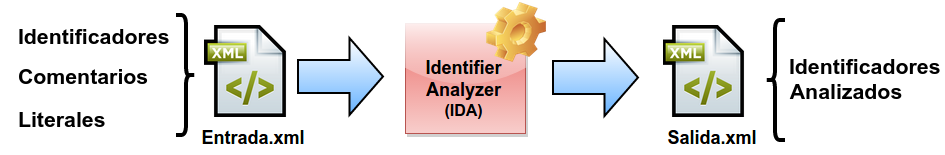
\includegraphics[scale= 0.57]{./ape/ape_01.png}
}
\caption{Extensión de IDA}
\label{arq1}
\end{figure}


\newpage

La invocación de IDA con un archivo XML se realiza a través del archivo JAR\footnote[1]{JAVA Archive.} (correspondiente a la herramienta), ejecutando la siguiente orden en la línea de comandos del sistema operativo\footnote[2]{Se recomienda utilizar los sistemas operativos Windows o Linux con \textit{java runtime enviroment} instalado}:


\begin{lstlisting}[style=BashInputStyle]
  java -jar IDA.java <argumento>
\end{lstlisting}


En $<$\textsf{argumento}$>$ se coloca la ruta donde se encuentra ubicado el archivo XML a procesar (un ejemplo en linux es \textsf{/home/entrada.xml}\footnote[3]{No es necesario que se llame entrada, pero si que tenga extensión xml.}). Este argumento no es obligatorio, y en caso de no pasarlo, se ejecuta la interfaz normal de IDA que fue descripta en el capítulo 4.
La herramienta IDA procesa el archivo XML ingresado ejecutando los algoritmos de análisis de ids que tiene implementados (Greedy, Samurai y Expansión Básica) y produce los resultados correspondientes a cada uno de ellos.
A continuación, se describe como debe estar estructurado el archivo XML de entrada.

\noindent \textbf{\\Archivo XML de Entrada\\} 

El archivo XML de entrada debe comenzar con \mbox{$<$\textsf{entrada}$>$} y finalizar con \mbox{$<$/\textsf{entrada}$>$} (Ver Figura \ref{xml1}), entre las etiquetas antes mencionadas se pueden especificar los siguientes elementos: 

\begin{description}
\itemsep0em%reduce espacio
\item[Lista de Identificadores:] Contiene los ids que van a ser analizados, se delimita con \mbox{$<$\textsf{lista\_ids}$>$} y \mbox{$<$/\textsf{lista\_ids}$>$}; cada elemento de esta lista se especifica con $<$\textsf{id}$>$ y $<$/\textsf{id}$>$; dentro de cada uno de estos elementos se coloca: el nombre del id con \mbox{$<$\textsf{nombre}$>$\textbf{nmId}$<$/\textsf{nombre}$>$}, y el número de línea con \mbox{$<$\textsf{linea}$>$\textbf{10}$<$/\textsf{linea}$>$} (Ver Figura \ref{xml1}).

\item[Lista de Frases:] Tiene las frases (asociadas a comentarios y literales) el inicio y fin de esta lista se indica con \mbox{$<$\textsf{lista\_frases}$>$} y \mbox{$<$/\textsf{lista\_frases}$>$};
cada elemento de esta lista se delimita con $<$\textsf{frase}$>$ y $<$/\textsf{frase}$>$; dentro de cada uno de estos elementos de la lista se especifica: la frase correspondiente con \mbox{$<$\textsf{texto}$>$\textbf{File System}$<$/\textsf{texto}$>$}, y el número de línea con \mbox{$<$\textsf{linea}$>$\textbf{19}$<$/\textsf{linea}$>$} (Ver Figura \ref{xml1}).

\item[Lista de Clases:] Esta lista contiene las clases que posee el programa, se delimita con \mbox{$<$\textsf{lista\_clases}$>$} y \mbox{$<$/\textsf{lista\_clases}$>$}; cada elemento de esta lista se indica con $<$\textsf{clase}$>$ y $<$/\textsf{clase}$>$; cada uno de estos elementos tiene: el nombre del método  \mbox{$<$\textsf{nombre}$>$\textbf{Person}$<$/\textsf{nombre}$>$}, el número de línea donde comienza la clase \mbox{$<$\textsf{linea\_inicio}$>$\textbf{7}$<$/\textsf{linea\_inicio}$>$}, y la línea donde finaliza la clase \mbox{$<$\textsf{linea\_fin}$>$\textbf{30}$<$/\textsf{linea\_fin}$>$} (Ver Figura \ref{xml1}). 

\item[Lista de Métodos:] Similar a la lista anterior pero para métodos, se delimita con \mbox{$<$\textsf{lista\_metodos}$>$} y \mbox{$<$/\textsf{lista\_metodos}$>$}; cada elemento de este listado se indica con $<$\textsf{metodo}$>$ y $<$/\textsf{metodo}$>$; en cada uno de estos elementos se coloca: el nombre del método \mbox{$<$\textsf{metodo}$>$\textbf{getPerson}$<$/\textsf{metodo}$>$}, la línea donde comienza el método \mbox{$<$\textsf{linea\_inicio}$>$\textbf{11}$<$/\textsf{linea\_inicio}$>$}, y la línea donde finaliza la método \mbox{$<$\textsf{linea\_fin}$>$\textbf{19}$<$/\textsf{linea\_fin}$>$} (Ver Figura \ref{xml1}).

\end{description}

Cabe aclarar, que los nombres de los ids (Ver Figura \ref{xml1}) son el único dato que necesita ser especificado de manera obligatoria en el archivo proporcionado a IDA (dado que son la principal fuente de análisis de IDA). Por otro lado, el resto de los datos: Métodos, Clases, Frases, números de líneas (de cualquier elemento), también son importantes, pero solo colaboran con el análisis de los ids y no son indispensables.
 
Luego de que IDA analiza los ids, el próximo paso es almacenar los resultados de cada ejecución en un nuevo archivo XML de salida que se describe en la siguiente sección.


%\begin{description}
%\itemsep0em%reduce espacio
%\item[Lista de ids analizados:] Cada elemento de la lista posee, el nombre del id analizado, la correspondiente división Greedy, Samurai y las expansiones desde Greedy y Samurai.
%\end{description}


\newpage
\begin{figure}[h!] %[h] para here [b] para bottom [t] para top
\begin{lstlisting}[language=xml, frame=single]
<entrada>
	<lista_ids>
		<id>
		    <nombre>nmId</nombre>
		    <linea>10</linea>
		</id>    
		<id>	    	
		    <nombre>fs</nombre>
		    <linea>12</linea>
		</id>    	    	    
	</lista_ids>
	<lista_frases>
		<frase>
			<texto>name identifier</texto>
			<linea>9</linea>
		</frase>
		<frase>
			<texto>file system</texto>
			<linea>19</linea>
		</frase>
	</lista_frases>
	<lista_clases>
		<clase>
			<nombre>Person</nombre>
			<linea_inicio>7</linea_inicio>
			<linea_fin>30</linea_fin>
		</clase>
	</lista_clases>
	<lista_metodos>
		<metodo>
			<nombre>getPerson</nombre>
			<linea_inicio>11</linea_inicio>
			<linea_fin>19</linea_fin>
		</metodo>				
	</lista_metodos>	
</entrada>

\end{lstlisting}
\caption{Ejemplo de Archivo XML de entrada.}
\label{xml1}
\end{figure}

\newpage

\noindent \textbf{Archivo XML de Salida\\}

El archivo de salida contiene los ids analizados por las distintas técnicas y se crea en la misma ubicación que el archivo XML pasado por entrada (siguiendo con el ejemplo de la sección anterior se creará en \textsf{/home/salida.xml}\footnote[1]{Si ya existe un archivo con el nombre salida.xml, el mismo se sobrescribirá.}). El inicio de este archivo XML se indica con \mbox{$<$\textsf{salida}$>$} y el fin con \mbox{$<$/\textsf{salida}$>$} (Ver Figura \ref{xml2}), en su interior posee la siguiente lista:

\begin{description}
\itemsep0em%reduce espacio
\item[Lista de Identificadores Analizados:] Esta lista contiene los ids incluyendo el análisis realizado en cada uno, el inicio y fin de esta lista se especifica con  $<$\textsf{lista\_analisis\_ids}$>$ y $<$/\textsf{lista\_analisis\_ids}$>$; cada elemento de la lista se indica con $<$\textsf{id}$>$ y $<$/\textsf{id}$>$; dentro de cada elemento de la lista se encuentra: el nombre del id analizado delimitado con \mbox{$<$\textsf{nombre}$>$\textbf{nmId}$<$/\textsf{nombre}$>$}, la división greedy del id se ubica entre \mbox{$<$\textsf{div\_greedy}$>$\textbf{nm-id}$<$/\textsf{div\_greedy}$>$}, la división samurai del id entre\\ \mbox{$<$\textsf{div\_samurai}$>$\textbf{nm-id}$<$/\textsf{div\_samurai}$>$}, la expansión desde greedy entre \mbox{$<$\textsf{exp\_greedy}$>$\textbf{name identifier}$<$/\textsf{exp\_greedy}$>$}, y la expansión desde samurai entre $<$\textsf{exp\_samurai}$>$\textbf{name identifier}$<$/\textsf{exp\_samurai}$>$ (Ver Figura \ref{xml2}).
\end{description}

\enlargethispage{\baselineskip}%agrega linea al final de la hoja.
\enlargethispage{\baselineskip}
\enlargethispage{\baselineskip}
\enlargethispage{\baselineskip}
\enlargethispage{\baselineskip}

\begin{figure}[h!]
\begin{lstlisting}[language=xml, frame=single]
<salida>
  <lista_analisis_ids>
    <id>
      <nombre>nmId</nombre>
      <div_greedy>nm-id</div_greedy>
      <div_samurai>nm-id</div_samurai>
      <exp_greedy>name identifier</exp_greedy>
      <exp_samurai>name identifier</exp_samurai>
    </id> 
    <id>
      <nombre>fs</nombre>
      <div_greedy>fs</div_greedy>
      <div_samurai>fs</div_samurai>
      <exp_greedy>file system</exp_greedy>
      <exp_samurai>file system</exp_samurai>
    </id>         
  </lista_analisis_ids>
</salida>
\end{lstlisting}
\caption{Ejemplo de Archivo XML de salida.}
\label{xml2}
\end{figure}

\end{appendices}


